\section{Methods}
\begin{frame}{Particle Filter Setup}
\begin{itemize}
    \item Weighting function
        \begin{itemize}
            \item Continuous, Long Tailed, Zero-Mean 
            \item Too wide $\rightarrow$ under-sensitivity, 
                slow or no convergence
            \item Too thin $\rightarrow$ reduces robustness 
                to noise, particle deprivation
            \item For this work, $N(0, 0.005^2)$ used
        \end{itemize}
    \item Resampling 
        \begin{itemize}
            \item Stratified Resampling can result in truncated tails 
                    on posterior
            \item Regularized Resampling can result in over smoothing and 
                    slow convergence
            \item Resampling Performed Rarely
        \end{itemize}
    \item Number of particles
        \begin{itemize}
            \item More particles give higher fidelity 
            \item Large Initial Particle Count (16000)
        \end{itemize}
    \item Prior Distribution
    \begin{itemize}
            \item Large $\tau$ parameters can oversmooth
            \item $\epsilon$ needs large variance
    \end{itemize}
\end{itemize}
\note{Because the first 20 measurements drop most weights very quickly this gives a large breadth,
    but after the initial calculations drops the computation requirements}
\note{This has not been done before}
\end{frame}

\begin{frame}
\begin{figure}[htbp]
\centering
% The state vector is represented by a blue circle.
% "minimum size" makes sure all circles have the same size
% independently of their contents.
\tikzstyle{state}=[circle, thick, minimum size=1.2cm,
                   draw=blue!80, fill=blue!20]

% The measurement vector is represented by an orange circle.
\tikzstyle{measurement}=[circle, thick, minimum size=1.2cm,
                         draw=orange!80, fill=orange!25]

% The control input vector is represented by a purple circle.
\tikzstyle{input}=[circle, thick, minimum size=1.2cm,
                   draw=purple!80, fill=purple!20]

% The input, state transition, and measurement matrices
% are represented by gray squares.
% They have a smaller minimal size for aesthetic reasons.
\tikzstyle{matrx}=[rectangle, thick, minimum size=1cm,
                   draw=gray!80, fill=gray!20]
\begin{tikzpicture}[>=latex,text height=1.5ex,text depth=0.25ex]
  \matrix[row sep=0.5cm,column sep=0.5cm] {
    % First line: Control input
    &
        \node (u_k-1) [input]{$\mathbf{u}_{k-1}$}; &
        &
        \node (u_k)   [input]{$\mathbf{u}_k$};     &
        &
        \node (u_k+1) [input]{$\mathbf{u}_{k+1}$}; &
        \\
        % Second line: System noise & input matrix
        \node (B_k-1) [matrx] {$\mathbf{B}$};       &
        \node (B_k)   [matrx] {$\mathbf{B}$};       &
        \node (B_k+1) [matrx] {$\mathbf{B}$};       &
        \\
        % Third line: State & state transition matrix
        \node (A_k-2)         {$\cdots$};           &
        \node (x_k-1) [state] {$\mathbf{x}_{k-1}$}; &
        \node (A_k-1) [matrx] {$\mathbf{A}$};       &
        \node (x_k)   [state] {$\mathbf{x}_k$};     &
        \node (A_k)   [matrx] {$\mathbf{A}$};       &
        \node (x_k+1) [state] {$\mathbf{x}_{k+1}$}; &
        \node (A_k+1)         {$\cdots$};           \\
        % Fourth line: Measurement noise & measurement matrix
        \node (H_k-1) [matrx] {$\mathbf{H}$};       &
        \node (H_k)   [matrx] {$\mathbf{H}$};       &
        \node (H_k+1) [matrx] {$\mathbf{H}$};       &
        \\
        % Fifth line: Measurement
        &
        \node (z_k-1) [measurement] {$\mathbf{z}_{k-1}$}; &
        &
        \node (z_k)   [measurement] {$\mathbf{z}_k$};     &
        &
        \node (z_k+1) [measurement] {$\mathbf{z}_{k+1}$}; &
        \\
    };

\end{figure}
\end{frame}

\begin{frame}{FMRI Noise}
\centering

Resting State Noise

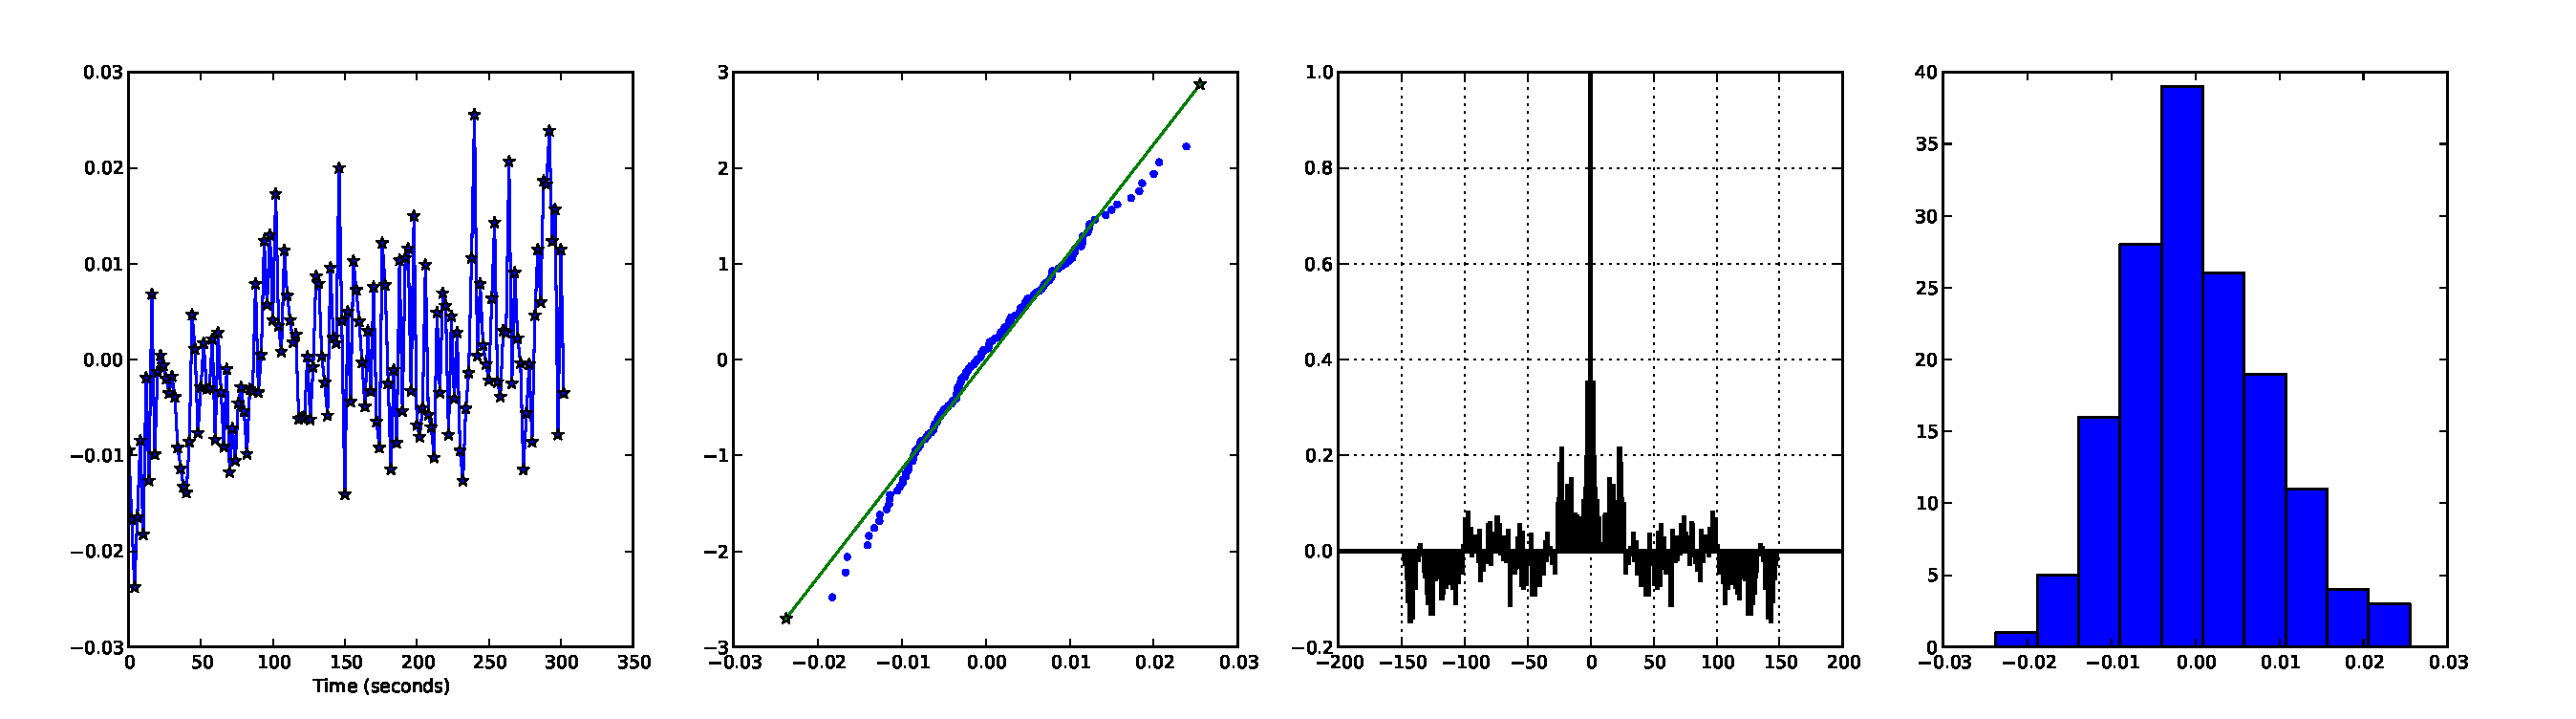
\includegraphics[trim=3cm 0cm 3cm 0cm,width=.75\textwidth]{noise2_0009_22_38_23}

Resting State Noise Steps

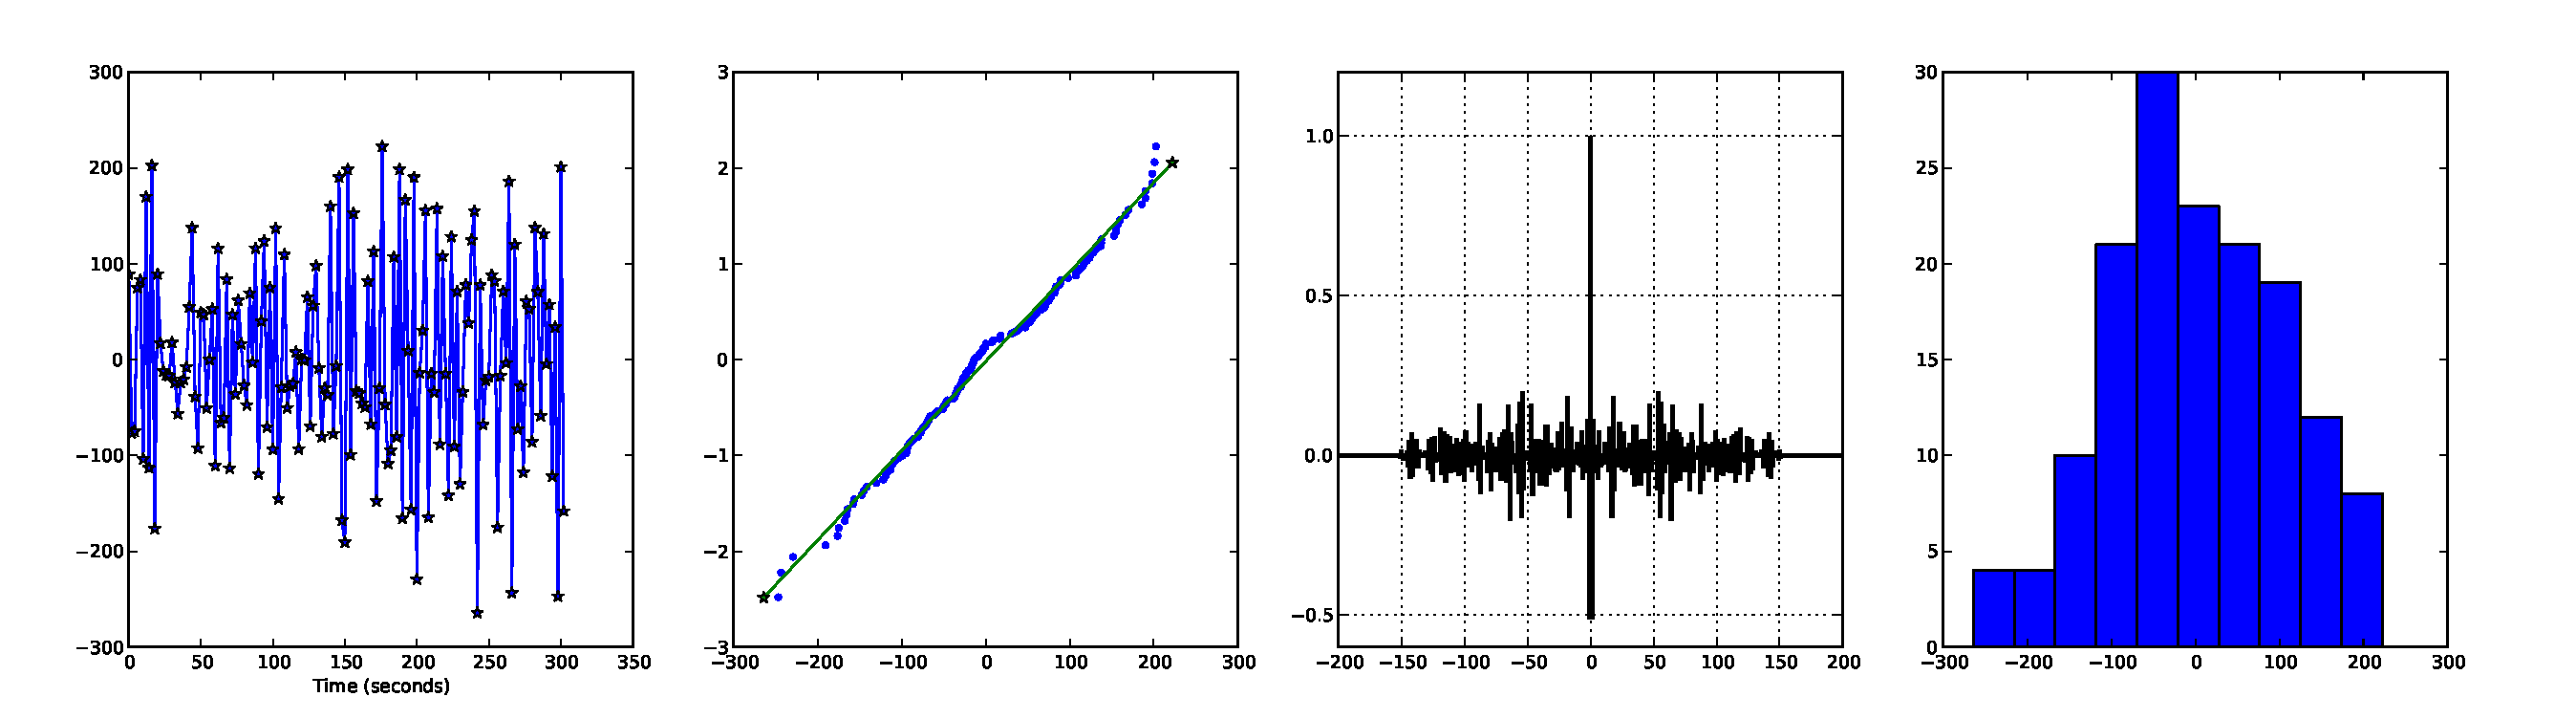
\includegraphics[trim=3cm 0cm 3cm 0cm,width=.75\textwidth]{noise2_0009d_22_38_23}

\note{Tanabe 2002 \autoref{Tanabe2002} 10-15\% of voxels exhibit significant drift}
\note{Occurs in Cadavers.}
\end{frame}

\begin{frame}{Preprocessing}
  \begin{columns}
    \begin{column}{.6\textwidth}
        \begin{itemize}
            \item Drop Initial Volumes (9, $18.9$s)
            \item Realign Over Time
            \item Detrend (SPM uses $1/128 Hz$ cut off)
            \item Gaussian Smoothing (SPM Only)
            \begin{itemize}
                \item Imposes Gaussianity
                \item Increases SNR
                \item Reduces Bonferroni Correction Requirement
            \end{itemize}
        \end{itemize}
    \end{column}
    
    \begin{column}{.4\textwidth}
        \includegraphics[width=\textwidth]{preprocess}
    \end{column}
  \end{columns}
\end{frame}

